\section{Facility Description}

\subsection{Location and Setting}

DreamLab is situated on a picturesque 5-acre plot in the Welsh countryside, offering:

\begin{itemize}
    \item Strategic location: 45 minutes from Cardiff, accessible to London (2.5 hours by train)
    \item Inspiring natural environment fostering creativity and focus
    \item Purpose-built facilities designed for immersive technology training
    \item High-speed fiber connectivity (10Gbps) enabling remote collaboration
    \item Secure campus with 24/7 access for residential programs
\end{itemize}

\subsection{Virtual Production Facility}

\subsubsection{LED Volume Stage}

\begin{labspec}
LED Wall System & 6m × 2.5m, 2.6mm pixel pitch, HDR & 1 & \pounds{180,000} \\
Disguise Media Servers & gx 2c servers with backup & 2 & \pounds{85,000} \\
Camera Tracking & Mo-Sys StarTracker system & 1 & \pounds{45,000} \\
Cinema Cameras & RED V-RAPTOR, ARRI Mini LF & 2 & \pounds{120,000} \\
Lighting Grid & ARRI SkyPanel, Aputure fixtures & Set & \pounds{35,000} \\
\end{labspec}

\subsubsection{Motion Capture Studio}

\begin{itemize}
    \item 12m × 8m capture volume with 24 Vicon cameras
    \item Full body and facial capture capabilities
    \item Real-time streaming to Unreal Engine and Unity
    \item Xsens MVN inertial suits for outdoor capture
    \item Props and rigging for performance capture
\end{itemize}

\subsection{Creative Technology Labs}

\subsubsection{Gaussian Splatting \& Neural Rendering Lab}

\begin{center}
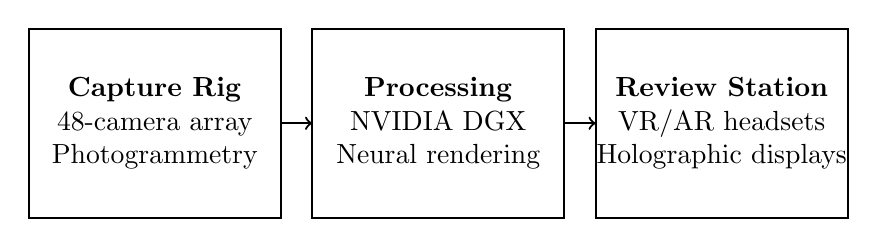
\begin{tikzpicture}[scale=0.8]
    % Capture Area
    \draw[thick] (0,0) rectangle (4,3);
    \node[align=center] at (2,1.5) {\textbf{Capture Rig}\\48-camera array\\Photogrammetry};
    
    % Processing Station
    \draw[thick] (4.5,0) rectangle (8.5,3);
    \node[align=center] at (6.5,1.5) {\textbf{Processing}\\NVIDIA DGX\\Neural rendering};
    
    % Review Area
    \draw[thick] (9,0) rectangle (13,3);
    \node[align=center] at (11,1.5) {\textbf{Review Station}\\VR/AR headsets\\Holographic displays};
    
    % Arrows showing workflow
    \draw[thick,->] (4,1.5) -- (4.5,1.5);
    \draw[thick,->] (8.5,1.5) -- (9,1.5);
\end{tikzpicture}
\end{center}

Equipment includes:
\begin{itemize}
    \item 48-camera photogrammetry array with synchronized capture
    \item NVIDIA DGX A100 for real-time neural rendering
    \item LiDAR scanning equipment (Leica BLK360)
    \item Holographic displays for 3D visualization
    \item Custom software pipeline for gaussian splatting workflows
\end{itemize}

\subsubsection{Telepresence \& XR Laboratory}

\begin{itemize}
    \item Microsoft HoloLens 2 development kits (10 units)
    \item Meta Quest Pro headsets with hand tracking (15 units)
    \item Varjo Aero professional VR headsets (5 units)
    \item Volumetric capture stage with depth cameras
    \item 5G private network for low-latency streaming
    \item Spatial audio system for immersive communication
\end{itemize}

\subsection{Engineering Simulation Visualization Suite}

\subsubsection{Hardware Infrastructure}

\begin{labspec}
Simulation Workstations & Threadripper PRO, RTX 4090, 128GB RAM & 8 & \pounds{64,000} \\
VR/AR Stations & High-end PCs with professional headsets & 6 & \pounds{36,000} \\
Visualization Wall & 4×4 4K display array & 1 & \pounds{25,000} \\
Haptic Devices & Force feedback for CAE interaction & 4 & \pounds{12,000} \\
\end{labspec}

\subsubsection{Software Ecosystem}

\begin{itemize}
    \item Engineering: Ansys, COMSOL, Simulink, SolidWorks
    \item Visualization: Unreal Engine, Unity, ParaView, EnSight
    \item Creative: Houdini, Nuke, DaVinci Resolve, Cinema 4D
    \item AI/ML: TensorFlow, PyTorch, CUDA toolkit, ComfyUI
    \item Collaboration: Perforce, Shotgrid, ftrack, Slack
\end{itemize}

\subsection{Drone Technology Center}

\subsubsection{Flight Training Area}

\begin{itemize}
    \item Indoor netted flight space (15m × 10m × 5m)
    \item Outdoor flight zone with CAA permissions
    \item Weather monitoring station
    \item Charging and maintenance stations
    \item Safety equipment and protocols
\end{itemize}

\subsubsection{Drone Fleet}

\begin{table}[H]
\centering
\begin{tabular}{lll}
\toprule
\textbf{Type} & \textbf{Models} & \textbf{Applications} \\
\midrule
Cinema Drones & DJI Inspire 3, FPV & Aerial cinematography \\
Mapping Drones & DJI M300 RTK, P4 RTK & Photogrammetry, surveying \\
Racing Drones & Custom 5" FPV builds & Pilot training, agility \\
Autonomous & PX4 development platforms & Computer vision, AI navigation \\
\bottomrule
\end{tabular}
\end{table}

\subsection{Supporting Infrastructure}

\subsubsection{Compute and Rendering Farm}

\begin{itemize}
    \item NVIDIA DGX A100 system for AI/ML training
    \item 20-node render farm with RTX 4090 GPUs
    \item 500TB high-speed storage array
    \item 10Gbps internal network with 100Gbps backbone
    \item Cloud burst capability to AWS/Azure
\end{itemize}

\subsubsection{Collaboration Spaces}

\begin{center}
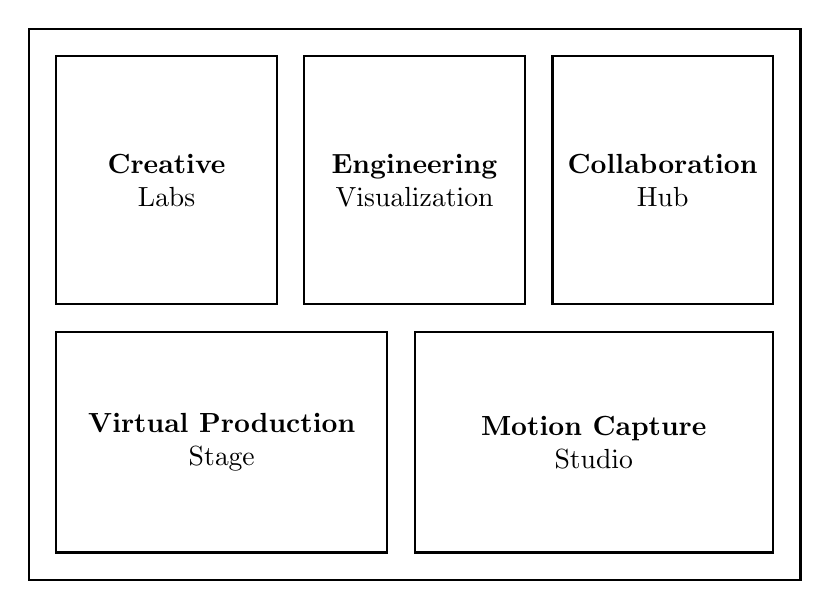
\begin{tikzpicture}[scale=0.7]
    % Main Building Layout
    \draw[thick] (0,0) rectangle (14,10);
    
    % VP Stage
    \draw[thick] (0.5,0.5) rectangle (6.5,4.5);
    \node[align=center] at (3.5,2.5) {\textbf{Virtual Production}\\Stage};
    
    % MoCap Studio
    \draw[thick] (7,0.5) rectangle (13.5,4.5);
    \node[align=center] at (10.25,2.5) {\textbf{Motion Capture}\\Studio};
    
    % Creative Labs
    \draw[thick] (0.5,5) rectangle (4.5,9.5);
    \node[align=center] at (2.5,7.25) {\textbf{Creative}\\Labs};
    
    % Engineering Suite
    \draw[thick] (5,5) rectangle (9,9.5);
    \node[align=center] at (7,7.25) {\textbf{Engineering}\\Visualization};
    
    % Collaboration Hub
    \draw[thick] (9.5,5) rectangle (13.5,9.5);
    \node[align=center] at (11.5,7.25) {\textbf{Collaboration}\\Hub};
\end{tikzpicture}
\end{center}

\subsection{Sustainable Features - Enhanced}

\subsubsection{Renewable Energy System}

\begin{solarroi}
\textbf{18kW Solar Installation with Battery Storage}

\begin{table}[H]
\centering
\begin{tabular}{lr}
\toprule
\textbf{Component} & \textbf{Specification} \\
\midrule
Solar Panels & 45x 400W panels (18kW total) \\
Battery Storage & 4x Tesla Powerwall (54kWh) \\
Annual Generation & 16,500 kWh estimated \\
Tech Load Offset & 60\% of compute/render power \\
Grid Independence & 40-50\% overall average \\
25-year Savings & \pounds{285,000} projected \\
\bottomrule
\end{tabular}
\end{table}
\end{solarroi}

\subsubsection{Sustainable Technology Practices}

\begin{itemize}
    \item GPU power management with workload scheduling
    \item Waste heat recovery for building heating
    \item Rainwater harvesting for cooling systems
    \item LED lighting throughout with motion sensors
    \item EV charging integrated with solar generation
\end{itemize}

\subsection{Accommodation Features - Tech Enhanced}

\subsubsection{Smart Residence Features}

The renovated Welsh farmhouse combines traditional charm with cutting-edge technology:

\begin{itemize}
    \item \textbf{Tech Amenities}: Gigabit WiFi, smart home automation, streaming studio
    \item \textbf{Work Spaces}: Private offices with dual 4K monitors, ergonomic furniture
    \item \textbf{Collaboration}: Video conferencing suite, brainstorming room with digital whiteboards
    \item \textbf{Wellness}: VR meditation room, biophilic design elements
    \item \textbf{Entertainment}: Home theater with Dolby Atmos, gaming lounge
\end{itemize}

\subsection{Accessibility and Inclusivity}

DreamLab is committed to universal design principles:

\begin{itemize}
    \item All facilities wheelchair accessible with automatic doors
    \item Height-adjustable workstations throughout
    \item Assistive technology including eye-tracking interfaces
    \item Sign language interpretation available
    \item Neurodiversity-friendly spaces with adjustable lighting/sound
    \item Gender-neutral facilities
\end{itemize}